\section{User Centered Design Approach}

\textsc{HistoGlobe} wanted to be helpful and usable for a specific target group: history teachers in schools. Therefore we looked for a school in the area of Weimar that could serve as a location for a field study. We found a school in Jena, 25 km east of Weimar, that offered us to develop an instance of \textsc{HistoGlobe} directly for the usage in class.

\begin{figure}[H]
  \centering
  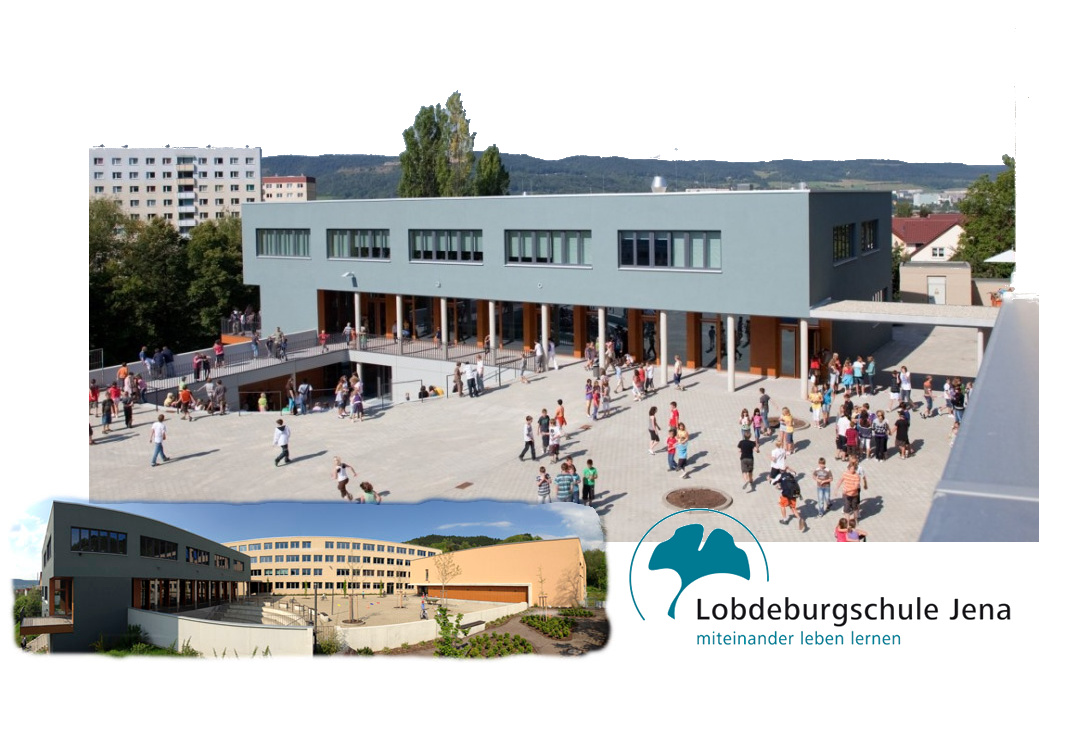
\includegraphics[width=0.7\textwidth]{graphics/lobdeburgschule.jpg}
\end{figure}

\paragraph{Lobdeburgschule} in Jena-Lobeda is a public school for all students from grade 1 to 13. A history teacher in grade 12 invited us to conduct a field study in his class to test \textsc{HistoGlobe} directly in school. This gave us the chance to develop the visualization in a User Centered Design approach thoughout the semester. Two members of the project group went every two or three weeks to the teacher in Jena in the time from October 2014 until April 2015. We presented new concepts, asked specific questions about the interface and the usage of the visualization in class and new problems and questions about the concept raised that had to be clarified until the next meeting.

\begin{figure}[H]
  \centering
  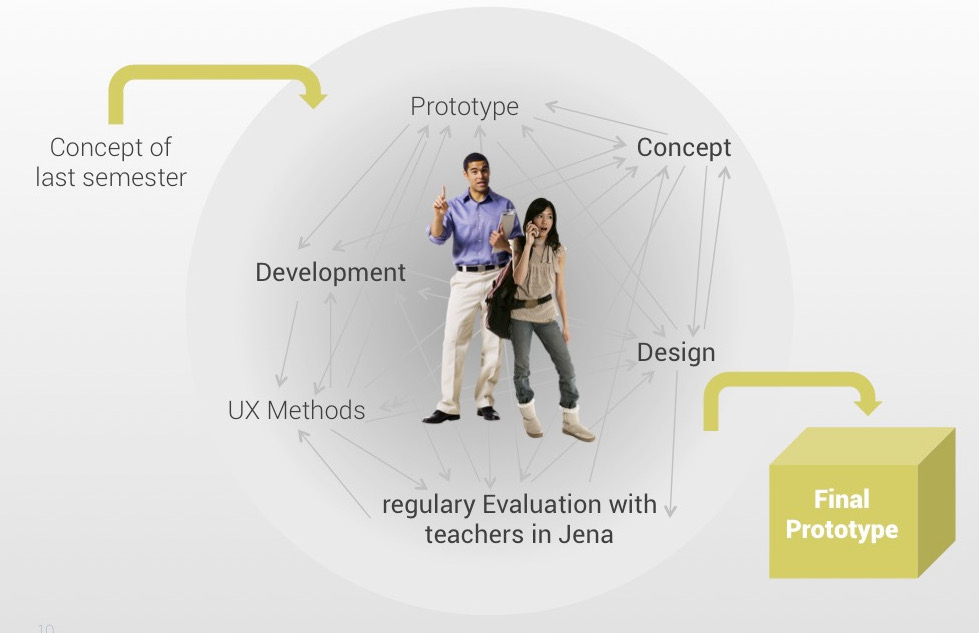
\includegraphics[width=0.7\textwidth]{graphics/design-1.jpg}
  \caption{User Centered Design}
\end{figure}

\subsection*{Design Iterations}
We had a lot of different design concepts. On the one hand we wanted to maximize the utility for the teacher to help him convey the necessary information in class but on the other hand design \textsc{HistoGlobe} in a way that we found suitable. We played around with orientation and the functionality of the timeline, the information about historical events on the map or the colors of the interface.

\begin{figure}[H]
  \centering
  \begin{minipage}{0.32\textwidth}
    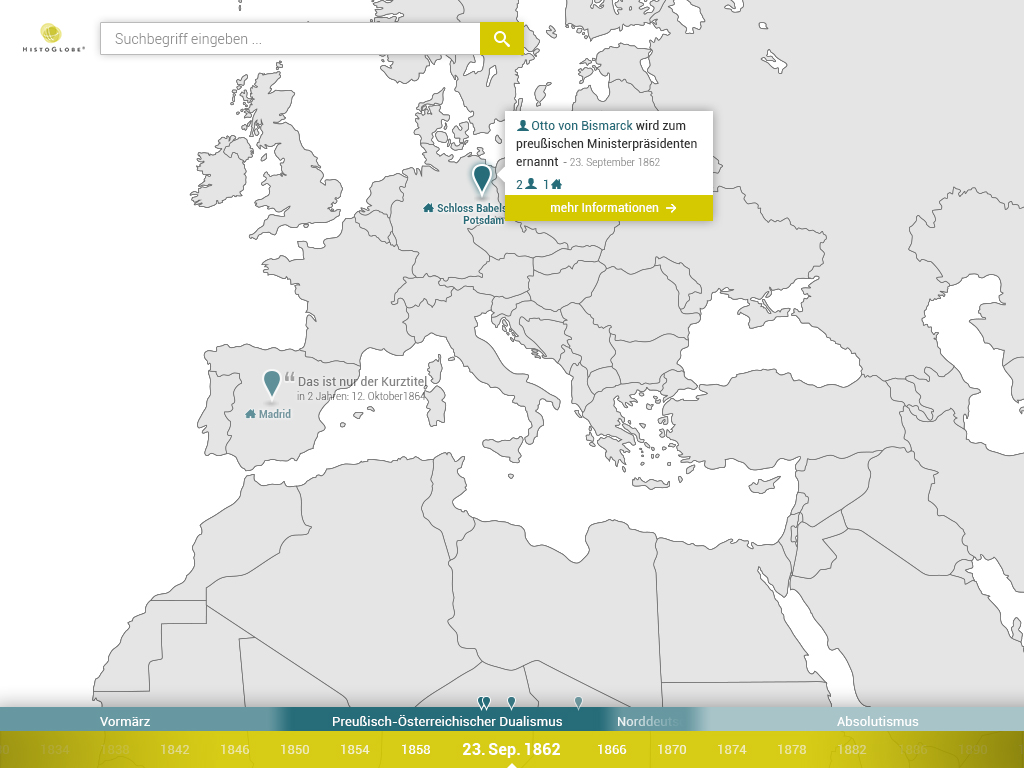
\includegraphics[width=0.95\textwidth]{graphics/design-2.jpg}
  \end{minipage}
  \begin{minipage}{0.32\textwidth}
    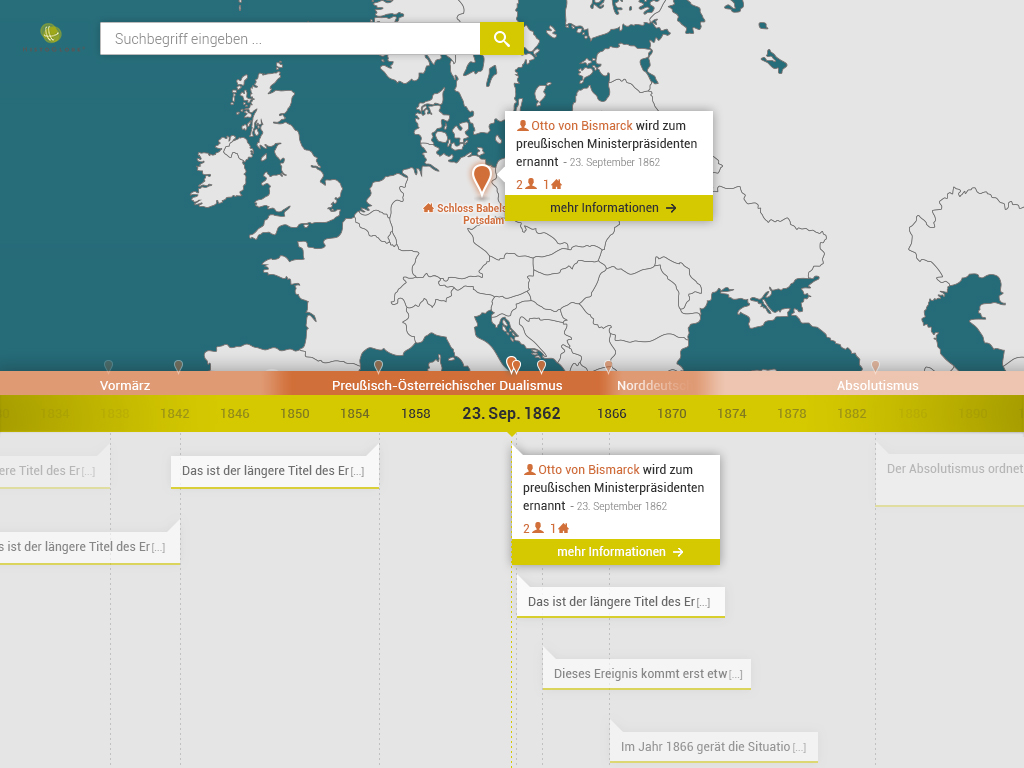
\includegraphics[width=0.95\textwidth]{graphics/design-3.jpg}
  \end{minipage}
  \begin{minipage}{0.32\textwidth}
    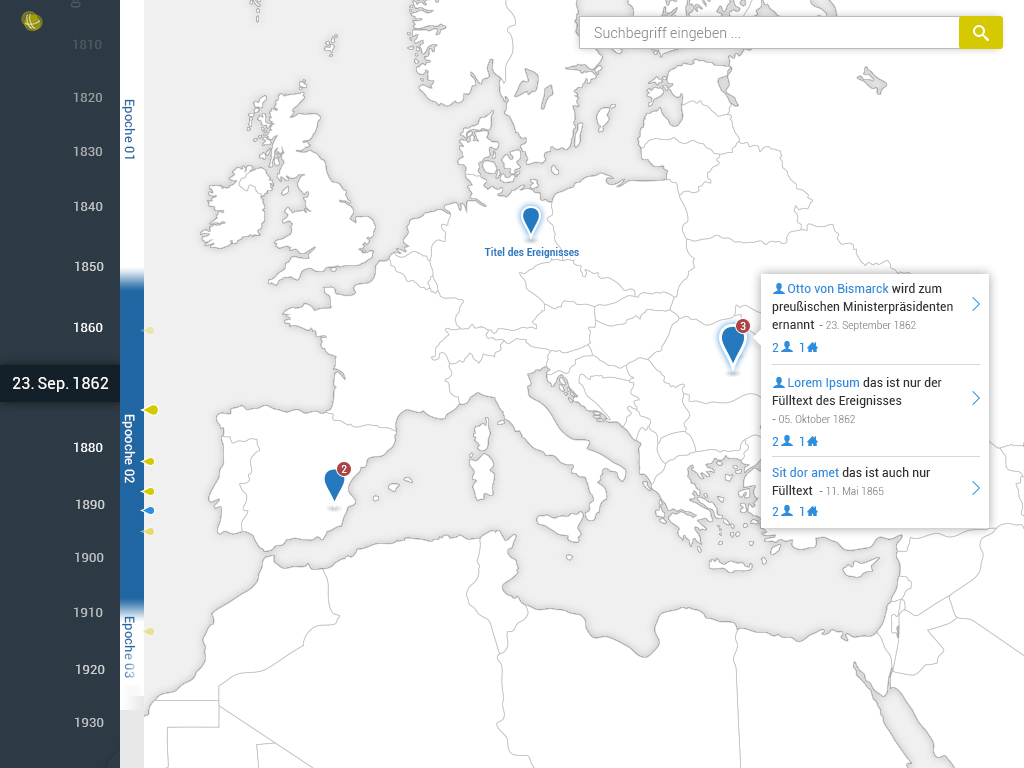
\includegraphics[width=0.95\textwidth]{graphics/design-4.jpg}
  \end{minipage}
  \caption{Several iterations of the design throughout the semester}
\end{figure}

In the next chapter we want to introduce the final elements of the user interface that were the result of the design iterations with the teacher.
